%\iffalse
\let\negmedspace\undefined
\let\negthickspace\undefined
\documentclass[journal,12pt,twocolumn]{IEEEtran}
\usepackage{cite}
\usepackage{amsmath,amssymb,amsfonts,amsthm}
\usepackage{algorithmic}
\usepackage{graphicx}
\usepackage{textcomp}
\usepackage{xcolor}
\usepackage{txfonts}
\usepackage{listings}
\usepackage{enumitem}
\usepackage{mathtools}
\usepackage{gensymb}
\usepackage{comment}
\usepackage[breaklinks=true]{hyperref}
\usepackage{tkz-euclide} 
\usepackage{listings}
\usepackage{gvv}                                        
\def\inputGnumericTable{}                                 
\usepackage[latin1]{inputenc}                                
\usepackage{color}                                            
\usepackage{array}                                            
\usepackage{longtable}                                       
\usepackage{calc}                                             
\usepackage{multirow}                                         
\usepackage{hhline}                                           
\usepackage{ifthen}                                           
\usepackage{lscape}

\newtheorem{theorem}{Theorem}[section]
\newtheorem{problem}{Problem}
\newtheorem{proposition}{Proposition}[section]
\newtheorem{lemma}{Lemma}[section]
\newtheorem{corollary}[theorem]{Corollary}
\newtheorem{example}{Example}[section]
\newtheorem{definition}[problem]{Definition}
\newcommand{\BEQA}{\begin{eqnarray}}
 \newcommand{\EEQA}{\end{eqnarray}}
\newcommand{\define}{\stackrel{\triangle}{=}}
\theoremstyle{remark}
\newtheorem{rem}{Remark}
\begin{document}
 \bibliographystyle{IEEEtran}
 \vspace{3cm}
 \title{\textbf{11.14-4}}
 \author{EE23BTECH11048-Ponugumati Venkata Chanakya$^{*}$% <-this % stops a space
 }
 \maketitle
 \newpage
 \bigskip
 \renewcommand{\thefigure}{\theenumi}
 \renewcommand{\thetable}{\theenumi}
 \textbf{QUESTION:}
 Which of the following functions of time represent (a) simple harmonic, (b) periodic
 but not simple harmonic, and (c) non-periodic motion? Give period for each case of
 peiodic motion ($\omega$ is any positive constant):\\
 \begin{enumerate}
 \item $\sin\brak{\omega t}-\cos\brak{\omega t}$\\
 \item $\sin^3\brak{\omega t}$\\
 \item $3\cos\brak{\frac{\pi}{4}- 2\omega t}$\\
 \item $\cos\brak{\omega t}+\cos\brak{3\omega t}+\cos\brak{5\omega t}$\\
 \item \text{exp}\brak{-\omega^2 t^2}\\
 \item $1+\omega t+\omega^2 t^2$\\
  \end{enumerate}
 \solution:\\
   Periodic function:
   \begin{align}
x(t+T) = x(t) \quad \forall x \in \mathbb{R}
\end{align}
 where min $T$ s.t $T>0$ is time period\\
 \\
    SHM:\\
    For a function to be in shm it must satisfy 
    \begin{align}
   \frac{d^2 x(t)}{dt^2} = - \alpha x\\
      \end{align}
   \begin{enumerate}
   \begin{table}[!ht]
    \centering
          \begin{tabular}{|c|c|c|} 
      \hline
\textbf{Variable}& \textbf{Description}& formula\\\hline
         $x(t)$&  Displacemen wrt mean position&none\\\hline
          $\omega$&Angular frequncy&$2\pi f$\\\hline
          $T$& Time period &none \\ \hline
          $\phi$& phase angle &none \\ \hline
    \end{tabular}

    \caption{input parameters}
    \label{tab:}
\end{table}
\item $\sin(2\pi f t)- \cos(2\pi f t)$\\
The function can be rewritten as:
 \begin{align}
  &= \sin(2\pi f t) - \sin\brak{\frac{\pi}{2} - 2\pi f t}\\
  &=2 \cos\brak{\frac{\pi}{4}} \sin\brak{2\pi f t - \frac{\pi}{4}}\\
  &=\sqrt{2}\sin\brak{2\pi f t - \frac{\pi}{4}}
 \end{align}
 \(\therefore\) SHM, \(T = \frac{1}{f}\) and \(\phi = \brak{\frac{-\pi}{4}}\) or \(\brak{\frac{7\pi}{4}}\)\\
 

     \item[(2)] $\sin^3(2\pi f t)$\\

 This function can be rewritten as\\ 
 \begin{align}
  &=\frac{1}{4}(3\sin(2\pi f t)-\sin(6\pi  f t))
 \end{align}
 $\therefore$ Periodic with period {T} = $\frac{1}{f}$ \\
\\

    \item[(3)] $3\cos\brak{\frac{\pi}{4}-4\pi f t}$\\

This function can be rewritten as\\ 
 \begin{align}
  =3\cos\brak{4\pi f t-\frac{\pi}{4}}\\
 \end{align}
 $\therefore$  SHM, $T = \frac{1}{2f}$  and  $\phi=\brak{\frac{-\pi}{4}}$ or $\brak{\frac{7\pi}{4}}$ \\
 \\

 \item[(4)]  $\cos(2\pi f t)+\cos(6\pi  f t)+\cos(10\pi  f t)$\\

This function can be rewritten as\\ 
 \begin{align}
  &=\cos(2\pi f t)+\cos(10\pi  f t)+\cos(6\pi  f t)\\
  &=2\cos\brak{\frac{2\pi f t+10\pi f t}{2}}\cos\brak{\frac{10\pi  f t-2\pi f t}{2}} +\cos(6\pi f t)\\
  &=2\cos(6\pi  f t) \cos(2\pi f t)+\cos(6\pi  f t)\\
  &=\cos(6\pi  f t) (1+2\cos(2\pi f t))
 \end{align}
 Period of $\cos(6\pi  f t)$ is $\frac{1}{3f}$\\ 
 Period of $1+2\cos(2\pi f t)$ is $\frac{1}{f}$\\ 
 Lcm is $\frac{1}{f}$\\
 $\therefore$  SHM,$T=$ $\frac{1}{f}$\\
 \\

 \item[(5)]  \text{exp}\brak{-(2\pi f)^2 t^2}\\

       \begin{center}
     As $T\to\infty$\\
    $\text{exp}\brak{-(2\pi f)^2 t^2}\to \infty$\\ 
       \end{center}
    $\therefore$  This never repeats and non periodic\\
    \\
    
 \item[(6)] $1+2\pi f t+(2\pi f)^2t^2$\\

 \begin{center}
  As $T\to\infty$\\
  $1+2\pi f t+(2\pi f)^2t^2  \to \infty$\\
  \end{center}
  $\therefore$ This never repeats and non periodic\\ 
 
\end{enumerate}
 \renewcommand{\thefigure}{\theenumi}
 \renewcommand{\thetable}{\theenumi}
 
 
 \begin{figure}[h!]
    \centering
    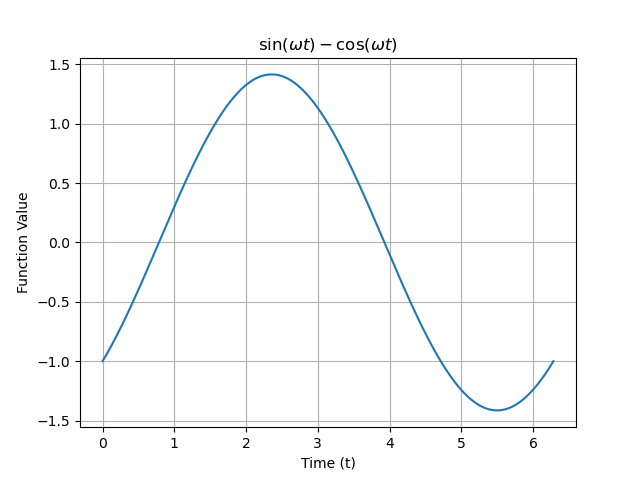
\includegraphics[width=0.4\textwidth]{figs/a1_fig1.png}
    \caption{$\sin(2\pi f t)- \cos(2\pi ft)$}
\end{figure}
 \begin{figure}[h!]
    \centering
    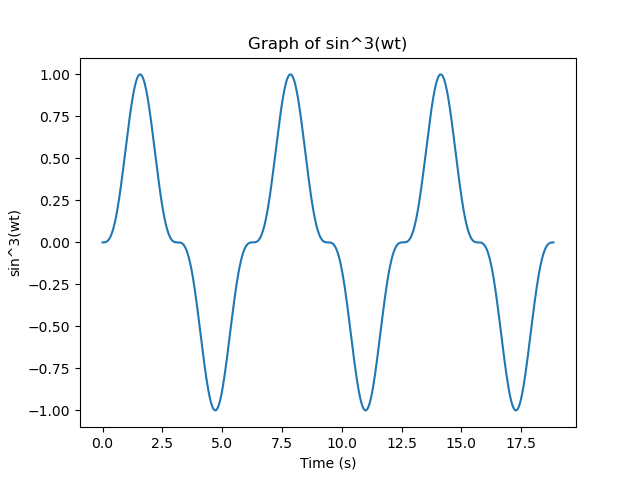
\includegraphics[width=0.4\textwidth]{figs/a1_fig2.png}
    \caption{$\sin^3(2\pi f t)$}
\end{figure}
\newpage
\begin{figure}[h!]
    \centering
    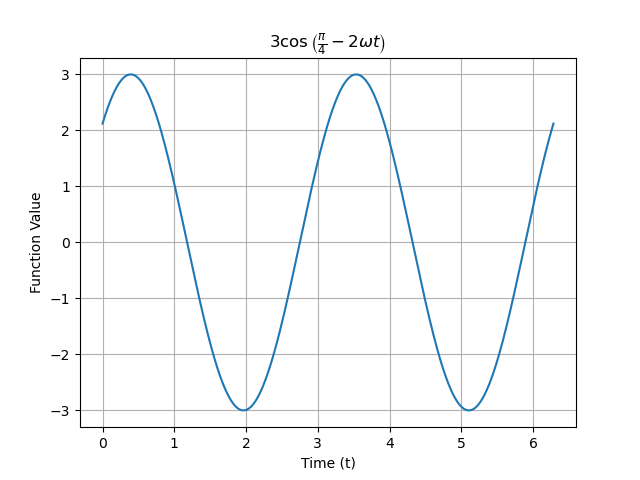
\includegraphics[width=0.4\textwidth]{figs/a1_fig3.png}
    \caption{$3\cos\brak{\frac{\pi}{4}- 4\pi f t}$}
\end{figure}
\begin{figure}[h!]
    \centering
    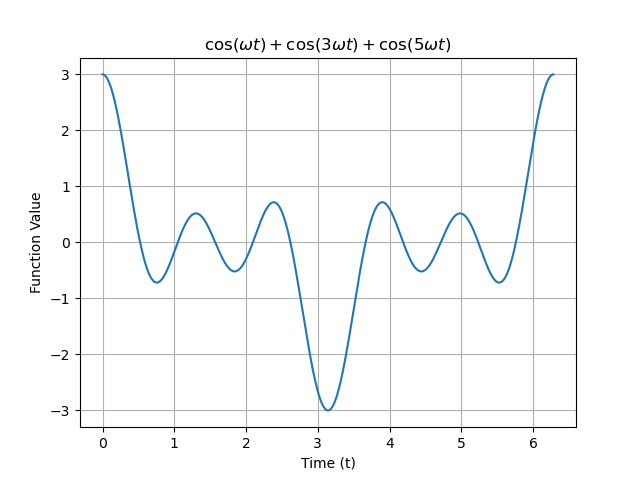
\includegraphics[width=0.4\textwidth]{figs/a1_fig4.png}
    \caption{$\cos(2\pi f t)+\cos(6\pi  f t)+\cos(10\pi  f t)$}
\end{figure}
\begin{figure}[h!]
    \centering
    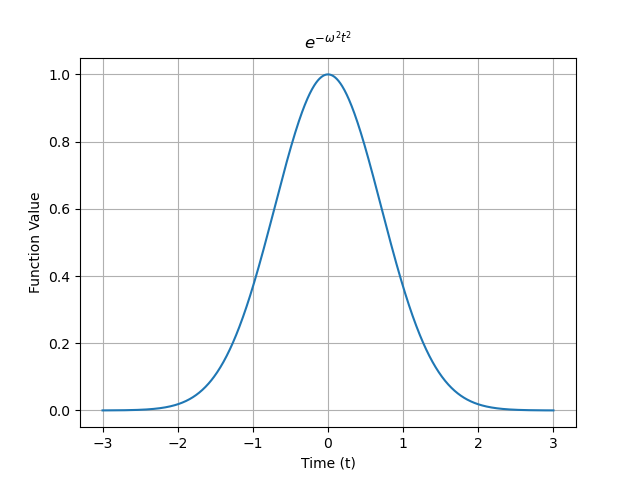
\includegraphics[width=0.4\textwidth]{figs/a1_fig5.png}
    \caption{$exp^{\brak{-(2\pi ft)^2}}$}
\end{figure}
\begin{figure}[h!]
    \centering
    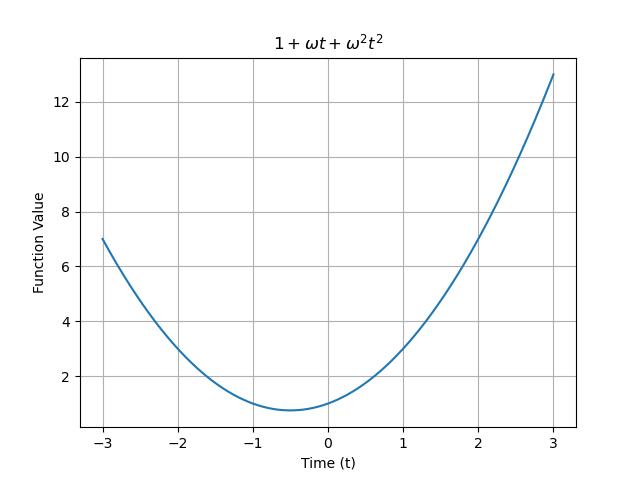
\includegraphics[width=0.4\textwidth]{figs/a1_fig6.png}
    \caption{$1+2\pi f t+(2\pi f t)^2$}
\end{figure}
\newpage
\begin{flushleft}
  \begin{table}[h]
   \def\arraystretch{1.5}:
   \caption{Summary}
   \label{tab:table.11.14-4}
    \begin{tabular}{|c|c|} 
      \hline
\textbf{Variable}& \textbf{Value}\\\hline
         $R_1$ & $2\ohm$\\\hline
          $R_2$ &$1\ohm$\\\hline
          $L_1$  &$2$ H \\ \hline
         $L_2$  &$0.5$ H \\ \hline
    \end{tabular}

  \end{table}
 \end{flushleft}
\end{document} 
